% -*- coding: UTF-8; -*-
%!TEX encoding = UTF-8
\documentclass[twoside,dvipsnames]{CUGThesis}

% 上方内容请勿动，完成了导入包与设置代码格式的工作

\title{机器学习课程报告} %报告题目
\subtitle{SVM多角度优化}
\author{毛郅皓} %作者姓名
\date{\today} %日期，默认当日
\school{计算机学院} %院系名称
\classnum{计算机科学与技术} %专业
\stunum {20231001111} %学号
\instructorone{万林} %指导教师1姓名
\instructoronelevel{副教授} %指导老师1职称
\logoname{Figures/School_Logo.png}
\headinfo{中国地质大学（武汉）}
\lineflag{no}%yes or no
\yearzh{2025}
\monthzh{5}

% \instructortwo{某某}
% \instructortwolevel{副教授}

\usepackage{makecell}
\usepackage{multicol}
\usepackage{multirow}
\usepackage{hyperref}

\begin{document}
	\maketitle
        %选择是否加入原创性声明
	% \makestatement

        %选择是否加入摘要
	% \begin{cnabstract}{关键词；关键词；关键词；关键词}
	% 	摘要
	% \end{cnabstract}
	
	% \begin{enabstract}{keyword; keyword; keyword; keyword}
	% 	abstract
	% \end{enabstract}

        %目录构造
	\makeToc

	
        \begin{spacing}{2}
		\section{引言}
	\end{spacing}


支持向量机（Support Vector Machine, SVM）作为一种经典的监督学习算法，在处理二分类问题中展现了卓越的泛化能力和数学严谨性，广泛应用于文本分类、图像识别、生物信息等多个领域。其核心思想是在特征空间中寻找一个最优超平面，以最大化两类样本之间的间隔，从而实现有效的分类任务。然而，尽管SVM在理论上具备较强的泛化能力，其在实际应用中仍面临许多挑战，亟需进一步的改进与优化。

首先，SVM的原始模型仅适用于线性可分问题，而对于非线性分布的数据，需要借助核方法进行特征空间的映射与转换。如何选择合适的核函数成为了SVM应用中的一个关键问题。其次，SVM对超参数（如惩罚系数 \(C\)、核函数参数 \(\gamma\) 等）非常敏感，不同参数组合可能会导致模型性能的显著差异，这对模型调优提出了较高的要求。此外，在高维数据或冗余特征的情况下，SVM的训练效率和分类性能可能会显著下降，进而引发所谓的“维度灾难”。因此，特征选择与降维技术在SVM的优化过程中扮演着至关重要的角色。

针对上述问题，本文从多个角度出发，对SVM进行了系统性的优化与改进，重点聚焦以下几个方面：

\begin{itemize}
    \item \textbf{特征优化策略}：通过主成分分析（PCA）降维处理线性相关特征、利用随机森林（RF）进行特征筛选，并在图像任务中引入神经网络编码器提取深层语义特征；
    \item \textbf{参数优化策略}：采用遗传算法（Genetic Algorithm）、模拟退火（Simulated Annealing）和贝叶斯优化等启发式策略，寻求更优的模型超参数组合；
    \item \textbf{损失函数策略}：尝试引入鲁棒性更强的替代损失函数，以提升模型对异常样本的适应能力；
    \item \textbf{集成学习策略}：采用投票（Voting）、自助采样（Bagging）和堆叠（Stacking）等集成学习方法，提升SVM在实际工程场景中的稳定性和鲁棒性。
\end{itemize}
当然并不是所有方法在本实验所选数据集中都起到了作用，有些效果并不明显，但后续会对其进行分析。

本实验通过以\textbf{Breast Cancer Wisconsin}和\textbf{螺旋形数据集}为基础，展开了一系列对比实验。通过可视化和量化指标，评估了各类优化手段对模型性能的影响。实验结果表明，结合合适的特征提取方式（如PCA + 随机森林特征选择）和核方法的优化策略，并辅以有效的超参数调优，SVM的分类性能得到了显著提升。尽管一些改进方法（如鲁棒损失函数）在某些场景下未能产生预期效果，但总体优化路径仍具有良好的可行性和推广价值。


        \newpage
        \begin{spacing}{2}
		\section{SVM基础与局限性分析}
	\end{spacing}
        \subsection{线性SVM数学基础}

在二分类问题中，设训练样本集为

\[
\mathcal{D} = \{(x_i, y_i)\}_{i=1}^n, \quad x_i \in \mathbb{R}^d, \quad y_i \in \{-1, +1\}
\]

SVM的目标是寻找一个超平面将正负样本分开。假设超平面的方程为

\[
f(x) = w^T x + b = 0 \tag{1}
\]

其中，\(w \in \mathbb{R}^d\) 是超平面的法向量，\(b\) 是偏置项。为了实现分类，我们要求所有训练样本满足如下约束条件：

\[
y_i(w^T x_i + b) \geq 1, \quad \forall i \tag{2}
\]

该约束确保正类样本位于超平面的正侧（\(y_i = +1\)），负类样本位于超平面的负侧（\(y_i = -1\)）。通过最大化正负类样本到超平面的间隔 \(\frac{2}{\|w\|}\)，SVM力求找到一个最优的超平面。

为最大化间隔，我们将优化问题转化为一个凸优化问题，目标是最小化

\[
\min_{w, b} \ \frac{1}{2} \|w\|^2 \quad \text{s.t.} \ y_i(w^T x_i + b) \geq 1, \quad \forall i \tag{3}
\]

其中，目标函数 \(\frac{1}{2} \|w\|^2\) 旨在最小化超平面的法向量的长度，从而最大化两类样本的间隔。

然而，实际数据往往包含噪声或不完全线性可分，因此引入松弛变量 \(\xi_i \geq 0\) 来允许部分样本位于超平面错误一侧，即引入“软间隔”概念。调整后的优化问题如下：

\[
\min_{w, b, \xi} \ \frac{1}{2} \|w\|^2 + C \sum_{i=1}^n \xi_i \quad \text{s.t.} \ y_i(w^T x_i + b) \geq 1 - \xi_i, \quad \forall i \tag{4}
\]

其中，\(C > 0\) 是惩罚因子，用于平衡间隔的大小和误分类的惩罚。较大的\(C\)值会使模型对误分类的容忍度降低，从而提升分类精度，但可能导致过拟合。

通过拉格朗日对偶性方法，将原始问题转化为对偶问题，从而便于引入核方法将问题扩展到非线性空间。我们可以定义拉格朗日函数为：

\[
L(w, b, \xi, \alpha) = \frac{1}{2} \|w\|^2 + C \sum_{i=1}^n \xi_i - \sum_{i=1}^n \alpha_i \left[ y_i(w^T x_i + b) - 1 + \xi_i \right] \tag{5}
\]

其中，\(\alpha_i \geq 0\) 是拉格朗日乘子。对拉格朗日函数求导并设置为零，得到最优解条件。最终的对偶问题形式为：

\[
\max_{\alpha} \sum_{i=1}^n \alpha_i - \frac{1}{2} \sum_{i=1}^n \sum_{j=1}^n \alpha_i \alpha_j y_i y_j x_i^T x_j \quad \text{s.t.} \ 0 \leq \alpha_i \leq C, \quad \sum_{i=1}^n \alpha_i y_i = 0 \tag{6}
\]

通过求解对偶问题，可以得到分类函数的最终形式：

\[
f(x) = \sum_{i=1}^n \alpha_i y_i x_i^T x + b \tag{7}
\]

其中，\(\alpha_i\) 是通过对偶问题优化得到的系数，最终的分类决策通过加权求和形式实现。

\begin{figure}[H]
		\centering
		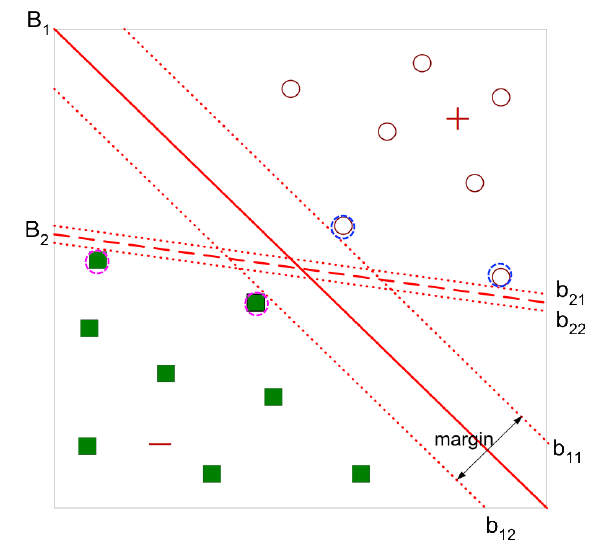
\includegraphics[scale=0.8]{Figures/img0.jpg}
		\caption{SVM求解示意图}
		\label{Fig:SVMExample}
\end{figure}




        

        \subsection{SVM可能的主要局限性}

尽管 SVM 具有较强的理论基础和实际效果，但在复杂数据环境中，仍存在一些主要局限性。在此部分，我们将详细讨论这些局限性及其可能的影响。

\subsubsection{非线性可分问题}

SVM 在处理线性可分数据时表现优秀，但在数据呈现明显非线性结构时，线性超平面无法实现有效分类。例如，当数据分布呈现“螺旋形”结构时，传统的 SVM 方法将无法划分数据。

对于非线性数据，SVM 的线性模型几乎完全失效，需要引入核函数来将数据映射到高维空间。通过这种方式，SVM 能够在高维空间中找到一个非线性超平面，实现对非线性数据的分类。

% 插入图片：非线性支持向量机示意图
\begin{figure}[H]
    \centering
    \includegraphics[scale=0.2]{Figures/image.png}  % 请根据实际路径修改
    \caption{非线性支持向量机示意图}
    \label{Fig:nonlinear_svm}
\end{figure}

通过核函数的帮助，SVM 将数据从原空间映射到高维空间，从而使得原本不可分的数据变得线性可分。常见的核函数包括高斯径向基函数（RBF）核、多项式核等。

\subsubsection{对核函数的依赖}

为了处理非线性问题，SVM 需要借助核函数 $K(x_i, x_j) = \phi(x_i)^T \phi(x_j)$，将样本映射到更高的维度。不同的核函数会根据数据的分布情况，选择不同的映射方式。常见的核函数有：

\begin{table}[H]
    \centering
    \caption{常用核函数}
    \label{Tab:Kernels}
    \scalebox{1.0}{
        \begin{tabular}{ccc}
            \toprule  % 表头上方粗线
            \textbf{名称} & \textbf{表达式} & \textbf{参数} \\
            \midrule  % 表头和数据之间的横线
            \textbf{线性核} & \( \kappa(x_i, x_j) = x_i^T x_j \) &  \\
            \textbf{多项式核} & \( \kappa(x_i, x_j) = (x_i^T x_j)^d \) & \( d \geq 1 \) 为多项式的次数 \\
            \textbf{高斯核} & \( \kappa(x_i, x_j) = \exp \left( -\frac{\|x_i - x_j\|^2}{2\sigma^2} \right) \) & \( \delta > 0 \) 为高斯核的带宽 (width) \\
            \textbf{拉普拉斯核} & \( \kappa(x_i, x_j) = \exp \left( -\frac{\|x_i - x_j\|}{\delta} \right) \) & \( \delta > 0 \) \\
            \textbf{Sigmoid核} & \( \kappa(x_i, x_j) = \tanh(\beta x_i^T x_j + \theta) \) & \( \tanh \) 为双曲正切函数, \( \beta > 0, \theta < 0 \) \\
            \bottomrule  % 表格底部粗线
        \end{tabular}

    }
    \vspace{10mm}
\end{table}

核函数的选择直接影响 SVM 的性能。不同的数据集可能适合不同的核函数，选择合适的核函数需要经验和数据特征的支持。然而，目前 SVM 并没有提供一个自动选择核函数的机制，往往需要通过交叉验证等方式手动选择。

% 插入图片：Polynomial 核函数图
\begin{figure}[H]
    \centering
    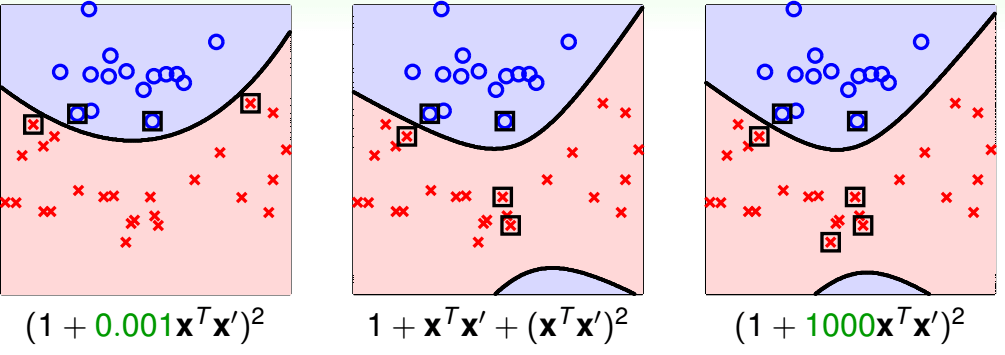
\includegraphics[scale=0.35]{assets/polynomial-kernel-function.png}  % 请根据实际路径修改
    \caption{Polynomial 核函数图示}
    \label{Fig:polynomial_kernel}
\end{figure}

% 插入图片：Gaussian 核函数图
\begin{figure}[H]
    \centering
    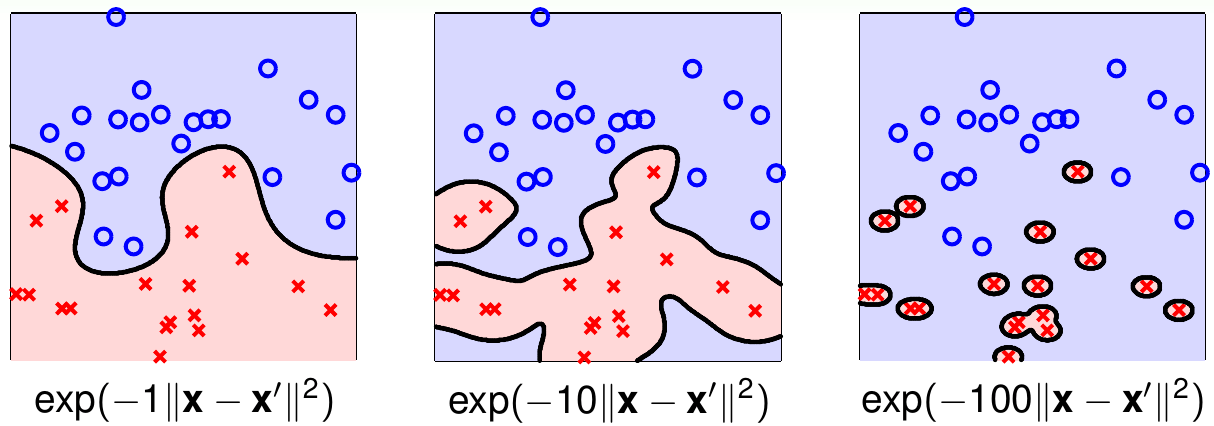
\includegraphics[scale=0.3]{assets/gaussian-kernel-function.png}  % 请根据实际路径修改
    \caption{Gaussian 核函数图示}
    \label{Fig:gaussian_kernel}
\end{figure}

不同的核函数具有不同的数学性质，适用于不同的数据结构。通过选择合适的核函数，SVM 可以在非线性数据上实现较好的分类效果。

\subsubsection{超参数调优困难}

SVM 模型的性能在很大程度上依赖于超参数的选择，主要包括惩罚因子 $C$、核函数参数 $\gamma$，以及多项式核的阶数等。这些超参数的选择直接影响到分类器的泛化能力和训练效果。

通过网格搜索等方法可以调整这些超参数，但这种方法往往计算量大，且调参效率低。过于依赖手动调参可能导致模型过拟合，从而影响模型的泛化能力。

% 插入图片：RBF SVM 超参数图
\begin{figure}[H]
    \centering
    \includegraphics[scale=0.6]{assets/rbf-svm-parameters-001.png}  % 请根据实际路径修改
    \caption{RBF 核 SVM 超参数调整}
    \label{Fig:rbf_svm_params}
\end{figure}

一般来说，$C$ 控制分类器对误分类的容忍度，较大的 $C$ 值会使得分类器对误差更敏感，导致过拟合；较小的 $C$ 值则可能导致欠拟合。$\gamma$ 是核函数的一个重要参数，控制了高维空间的映射程度。通过调整这些超参数，可以在训练集上获得较好的表现，但仍需小心过拟合。

\subsubsection{高维特征带来的维度灾难}

在处理高维数据时，SVM 的训练时间会显著增加，且随着支持向量的数量增加，模型的训练复杂度也会增大。高维空间中的数据会增加计算的难度，导致训练时间过长。同时，数据的维度越高，支持向量的数量也会增多，从而影响模型的泛化能力。

为了解决这个问题，特征选择和降维策略显得尤为重要。合理的特征选择可以有效减少数据维度，从而减少计算复杂度，并提高模型的性能。

% 插入图片：高维数据导致的维度灾难图
\begin{figure}[H]
    \centering
    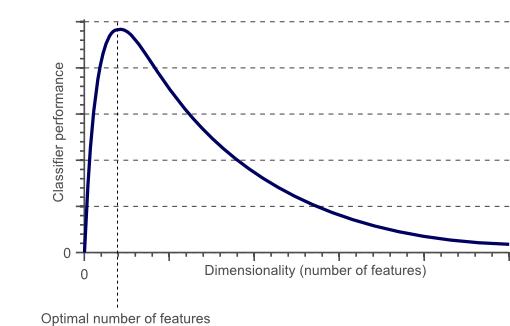
\includegraphics[scale=0.5]{assets/241651175178616.png}  % 请根据实际路径修改
    \caption{高维数据的维度灾难示意图}
    \label{Fig:high_dimensional_data}
\end{figure}

常用的降维方法如主成分分析（PCA）和线性判别分析（LDA）可以有效降低数据维度，从而加速训练过程并提高模型的泛化能力。

 在接下来的部分，将从特征工程、参数优化、损失函数、集成学习等方面入手，考虑解决这些局限性问题。

        



        \newpage
        \begin{spacing}{2}
		\section{特征优化策略及其实验}
	\end{spacing}


\section{特征优化方法与实验分析}

在支持向量机的实际应用中，特征的维度与质量直接影响模型的分类能力、泛化性能和计算效率。特征优化旨在通过对特征空间进行有效变换或选择，提升模型的表现。在复杂的非线性、高维特征场景下，特征优化的策略尤为重要。为了探索在这些情况下的有效优化方法，本节以人工生成的“噪声螺旋线数据集”为基准测试平台，围绕 \textbf{PCA 降维}、\textbf{核方法引入}、\textbf{随机森林特征选择}、\textbf{深度学习特征编码器}四种策略展开消融实验，系统评估各优化手段对 SVM 性能的影响。

\subsection{数据集构建与实验设置}

本实验设计使用可控结构的\textbf{双螺旋线数据集}作为测试基础，具备以下特征：

\begin{itemize}
    \item 原始数据为二维结构，构成典型非线性可分分类任务；
    \item 为模拟真实数据中的“维度灾难”问题，向每个样本随机添加10维高斯白噪声+线性变换；
    \item 最终数据维度为12维，其中2维为结构性主成分，10维为非判别性噪声维度。
\end{itemize}

数据集构建过程具体使用如下公式：

\[
\mathbf{x} = \mathbf{A} \cdot \mathbf{z} + \mathbf{N}
\]

其中，$\mathbf{x}$ 是带有噪声的样本，$\mathbf{A}$ 是线性变换矩阵，$\mathbf{z}$ 是原始数据的特征向量，而 $\mathbf{N}$ 是高斯白噪声。通过这个过程，模拟了在高维情况下特征的冗余和噪声影响。

\begin{figure}[H]
    \centering
    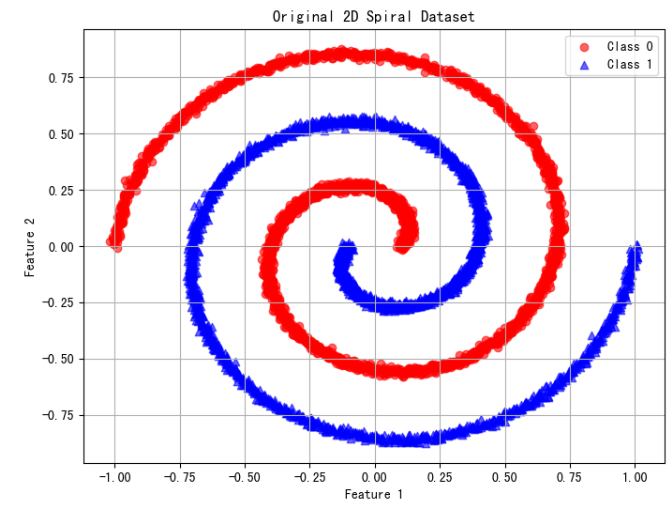
\includegraphics[scale=0.5]{assets/image-20250505233151486.png}
    \caption{示例图1}
    \label{Fig:example1}
\end{figure}

\begin{figure}[H]
    \centering
    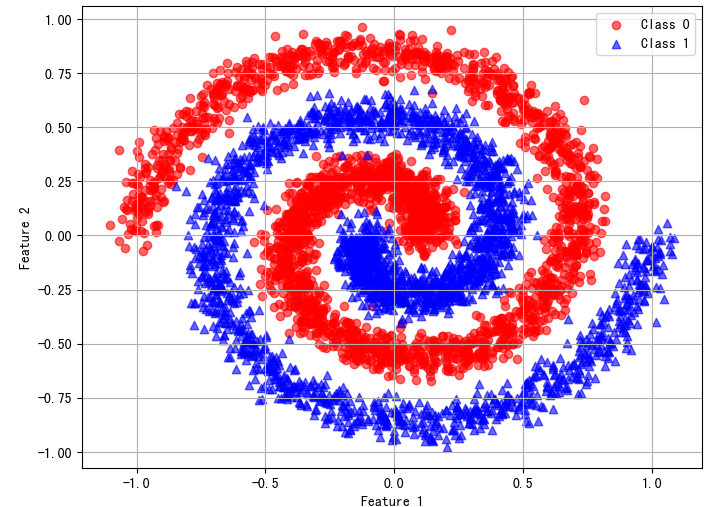
\includegraphics[scale=0.5]{assets/image-20250505233351045.png}
    \caption{示例图2}
    \label{Fig:example2}
\end{figure}

分类模型均采用 \textbf{支持向量机（SVM）} 作为主干，基础对比方法为线性核 SVM。所有实验统一使用训练集与测试集比例为 80\% : 20\%，采用训练准确率与训练耗时两项指标进行性能评估。

\subsection{消融实验设计}

为系统评估不同特征优化策略对支持向量机性能的影响，设计了如下多组组合实验。所有方案均以线性SVM为基础构建，逐步引入不同特征优化组件（PCA、核方法、随机森林选择、深度编码器）进行消融分析。

\begin{table}[H]
    \centering
    \caption{消融实验设计}
    \label{Tab:ablations}
    \scalebox{0.85}{
        \begin{tabular}{ccc c c}
            \toprule  % 表头上方粗线
            \textbf{编号} & \textbf{实验名称} & \textbf{是否PCA} & \textbf{是否核方法} & \textbf{是否RFSelect} \\
            \midrule  % 表头和数据之间的横线
            A    & 原始 SVM                     & ×       & ×          & ×            \\
            B    & PCA + 线性 SVM               & √       & ×          & ×            \\
            C    & PCA + 核方法 SVM             & √       & √          & ×            \\
            D    & RFSelect + 核方法 + SVM     & ×       & ×          & √            \\
            E    & PCA + DL编码器 + 核方法 +SVM & √       & ×          & ×            \\
            F    & PCA + RFSelect + 核方法 SVM  & √       & √          & √            \\
            \bottomrule  % 表格底部粗线
        \end{tabular}
    }
    \vspace{10mm}
\end{table}
在消融实验设计中，加入了不同的特征优化策略（如 PCA 降维，核方法等），通过实验逐步消除每个优化步骤对 SVM 性能的影响。这个过程可用以下公式来描述特征优化：

\[
\mathbf{x}_{opt} = f(\mathbf{x}; \text{PCA}, \text{RFSelect}, \text{Kernel})
\]

其中，$\mathbf{x}$ 表示原始特征，$f$ 表示特征优化过程，包含 PCA 降维、随机森林特征选择及核方法等步骤。

\subsection{实验结果及分析}

\begin{figure}[H]
    \centering
    \includegraphics[scale=0.3]{assets/image-20250506004453687.png}
    \caption{实验结果图1}
    \label{Fig:result1}
\end{figure}

\begin{figure}[H]
    \centering
    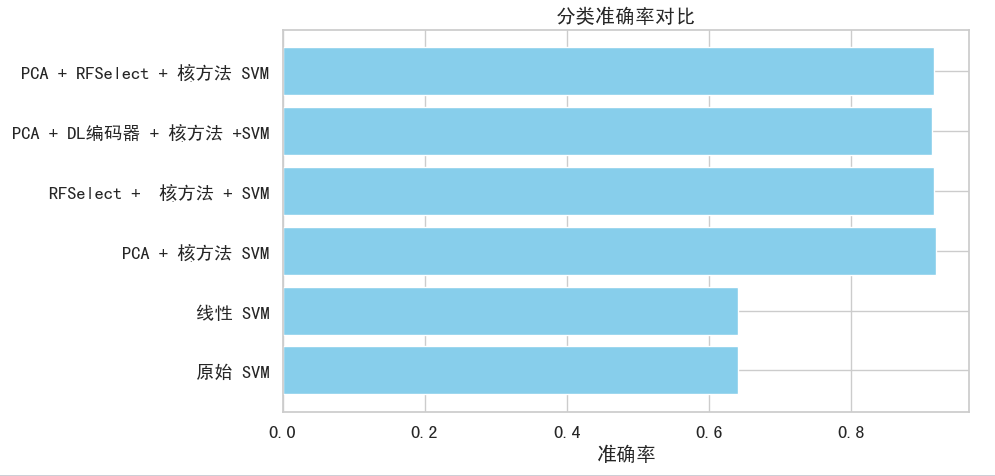
\includegraphics[scale=0.4]{assets/image-20250506004516826.png}
    \caption{实验结果图2}
    \label{Fig:result2}
\end{figure}

\begin{figure}[H]
    \centering
    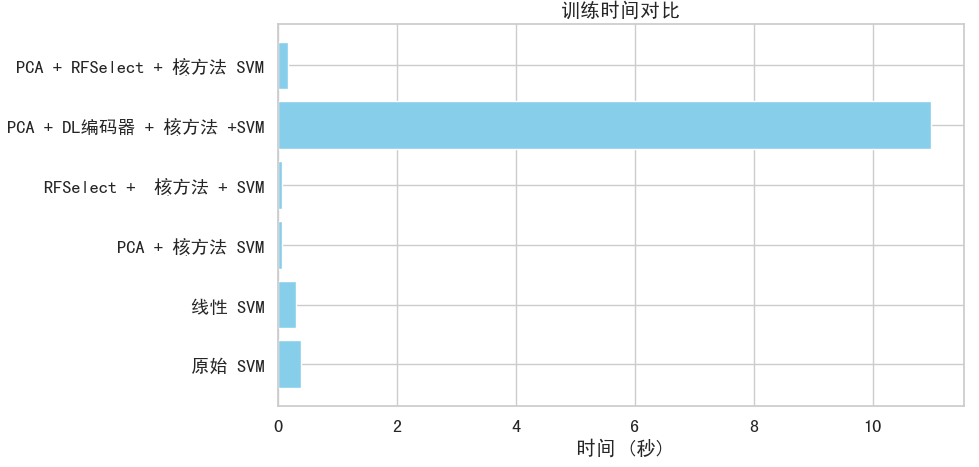
\includegraphics[scale=0.4]{assets/image-20250506004532589.png}
    \caption{实验结果图3}
    \label{Fig:result3}
\end{figure}

分析实验效果，我们可以看出，核方法起到了非常重要的作用。PCA并没有特别明显的改进。特征提取方法也没有很好的效果。对此我觉得可能是实现数据过于简单。但是降低维度确实对训练速度起到了很重要的作用。而由于DL编码器的使用，导致训练时间增加明显。随后改用makeclassification生成更复杂的数据进行实验。

\subsection{使用更复杂的数据}

\textbf{实验设计}
\begin{table}[H]
    \centering
    \caption{更复杂数据实验设计}
    \label{Tab:complex_data}
    \scalebox{0.85}{
        \begin{tabular}{ccc c}
            \toprule  % 表头上方粗线
            \textbf{实验编号} & \textbf{特征提取方法} & \textbf{分类模型}  & \textbf{目标} \\
            \midrule  % 表头和数据之间的横线
            1        & 原始特征               & 线性SVM  & 验证原始特征。 \\
            2        & PCA（降维至5维）       & RBF核SVM & 验证PCA降维性能。 \\
            3        & 随机森林特征选择（5个特征） & RBF核SVM & 验证特征选择提升性能。 \\
            4        & 自编码器（深度特征，5维）   & RBF核SVM & 验证深度学习特征。 \\
            5        & 原始特征               & MLP分类器 & 验证MLP性能。 \\
            \bottomrule  % 表格底部粗线
        \end{tabular}
    }
    \vspace{10mm}
\end{table}

这里给出数据分布以及随机森林特征重要性，且数据分布也是`1:1`的，为均衡分布。

\begin{figure}[H]
    \centering
    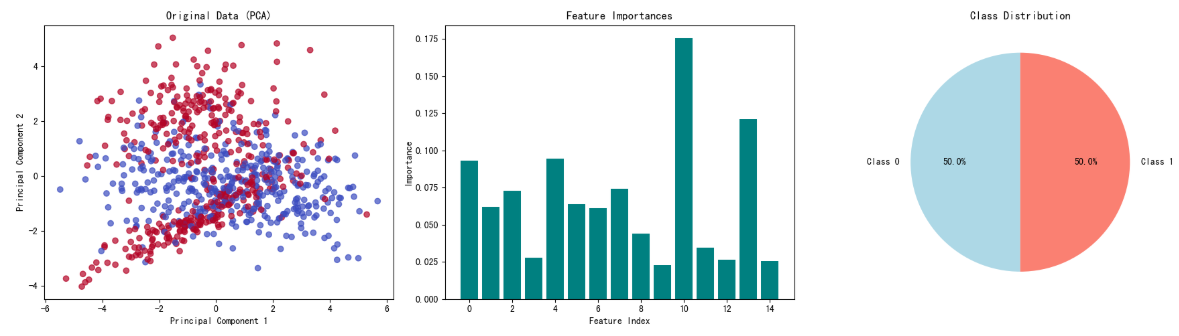
\includegraphics[scale=0.3]{assets/image-20250506005312094.png}
    \caption{数据分布与特征重要性}
    \label{Fig:data_distribution}
\end{figure}

在分析最终的准确率，可以发现随机森林特征选择体现出了更好的性能，虽然与直接的深度学习算法比其性能略有差距。

\begin{figure}[H]
    \centering
    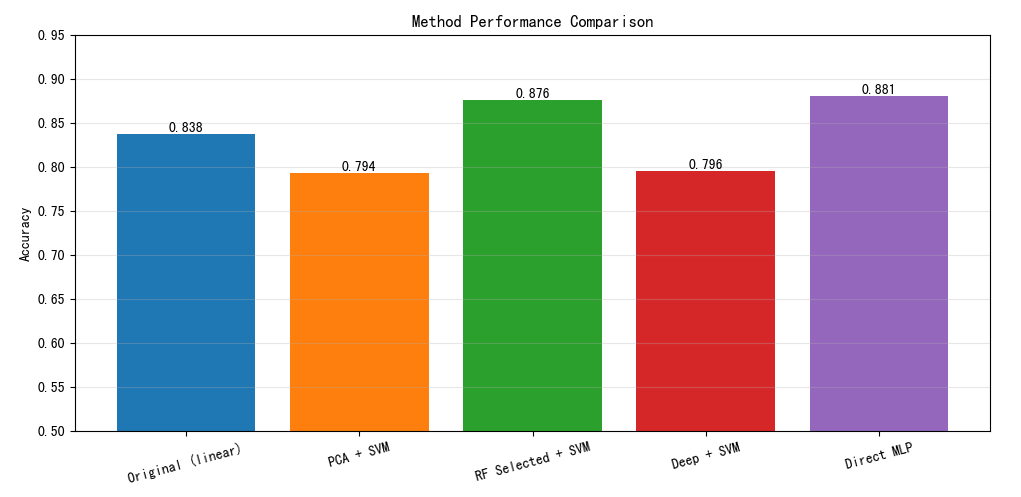
\includegraphics[scale=0.3]{assets/image-20250506005704472.png}
    \caption{最终准确率分析}
    \label{Fig:accuracy_analysis}
\end{figure}

\subsection{特征优化实验总结}

针对上方实验结果分析，对于简单实验效果并不好，但可以得到核方法起到关键性作用的结论。而对于复杂的数据，均使用了核方法，可以看到PCA+SVM反而降低了性能，而使用RF Selected+SVM方法起到了明显的增益效果。虽然在本实验中直接的深度学习方法效果更好，但是本课程是机器学习而非深度学习，我们不做讨论。


        
        

        
        \newpage
        \begin{spacing}{2}
		\section{超参数优化策略及其实验}
	\end{spacing}


        \subsection{数据预处理}

有第三小节实验，统一选择随机森林特征选择+核方法作为特征处理方式，使用 `Breast Cancer Wisconsin (Diagnostic)` 数据集进行实验。

这里给出不同分类器在该数据集上的表现，来源自 UCI 数据集：

\begin{figure}[H]
    \centering
    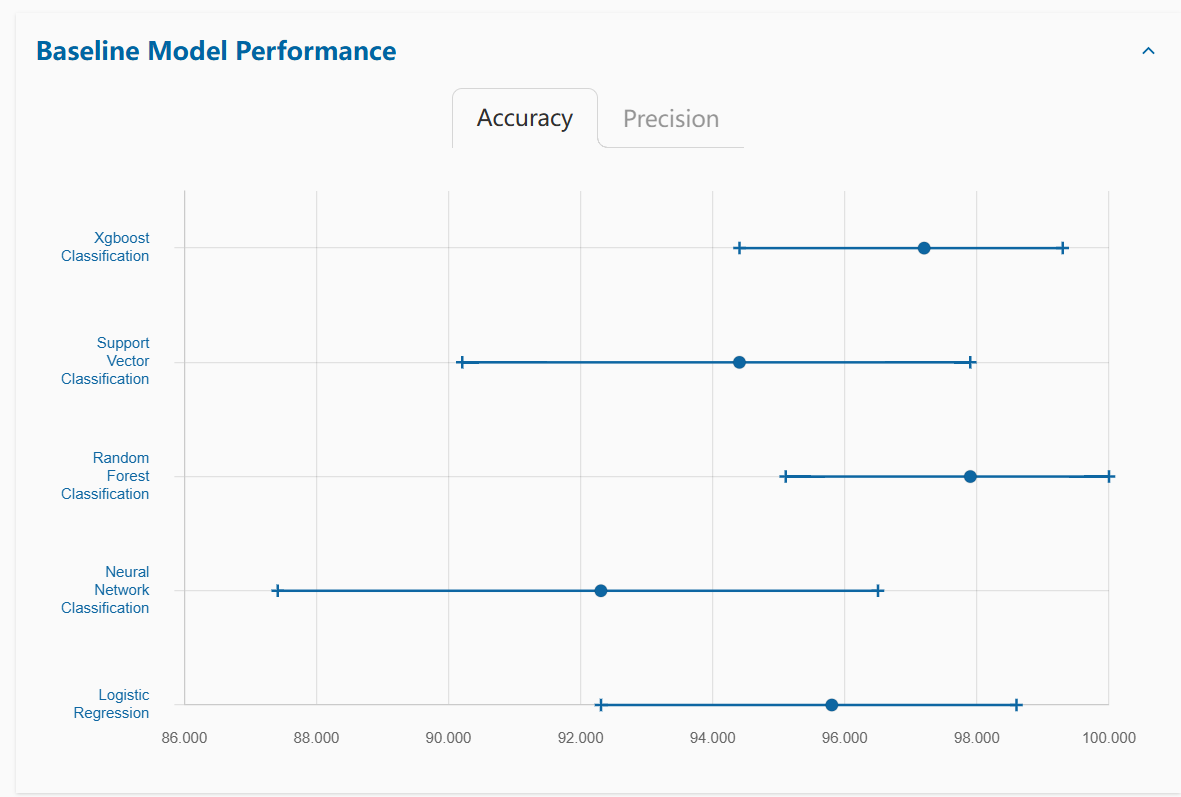
\includegraphics[scale=0.25]{assets/image-20250506021359884.png}
    \caption{不同分类器在乳腺癌数据集上的表现}
    \label{Fig:classifierPerformance}
\end{figure}

接下来展示数据处理过程。首先对数据分布进行展示，有离群点较多的特征，部分数据整体呈现偏态。

\begin{figure}[H]
    \centering
    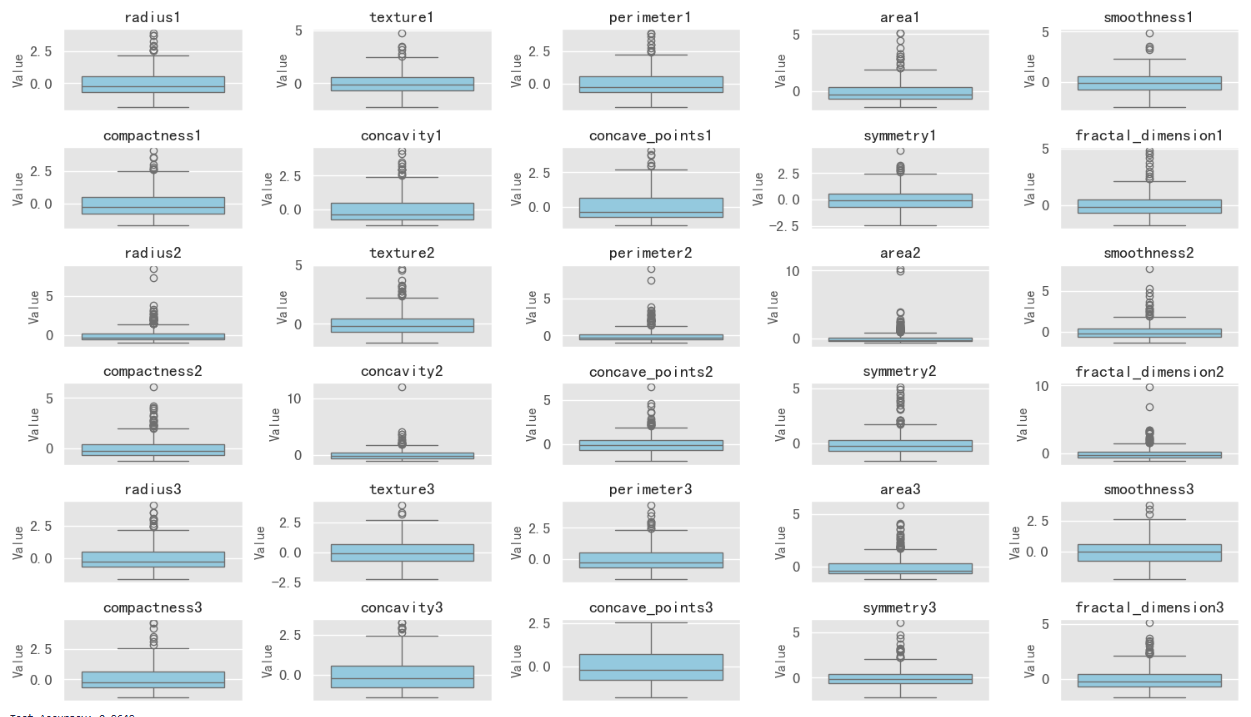
\includegraphics[scale=0.3]{assets/image-20250506012825516.png}
    \caption{数据分布展示1（离群点）}
    \label{Fig:dataDistribution1}
\end{figure}

\begin{figure}[H]
    \centering
    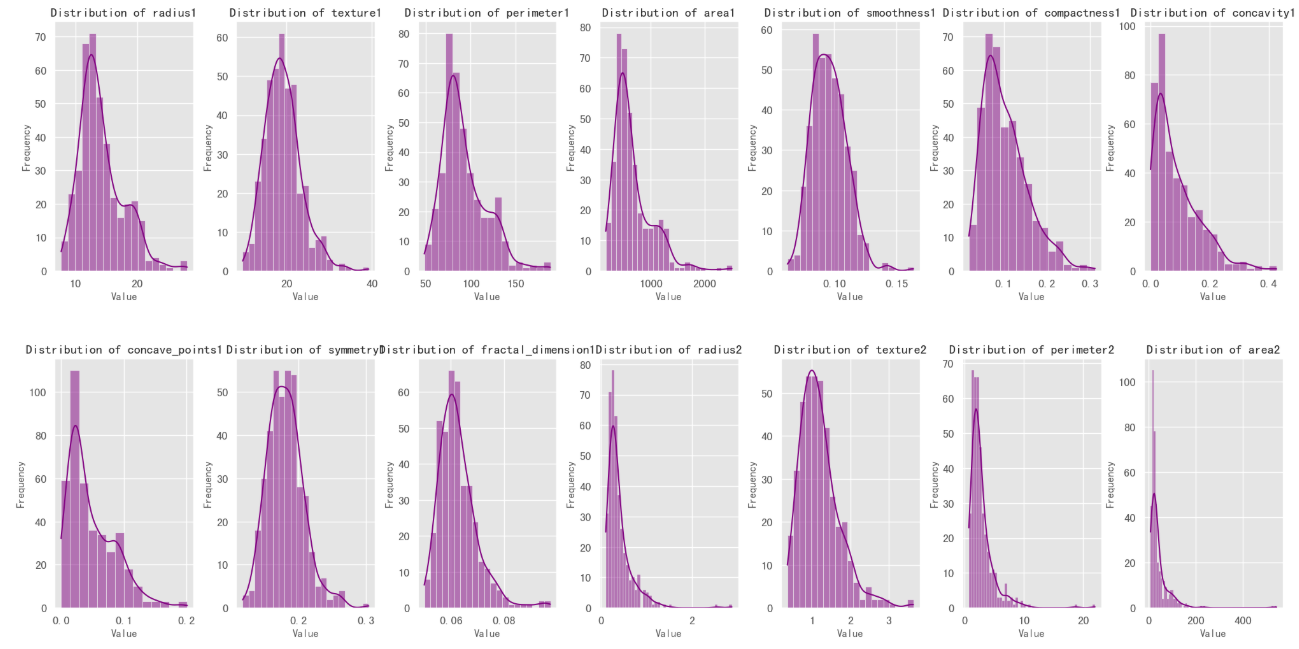
\includegraphics[scale=0.3]{assets/image-20250506013045512.png}
    \caption{数据分布展示2（偏态）}
    \label{Fig:dataDistribution2}
\end{figure}

\begin{figure}[H]
    \centering
    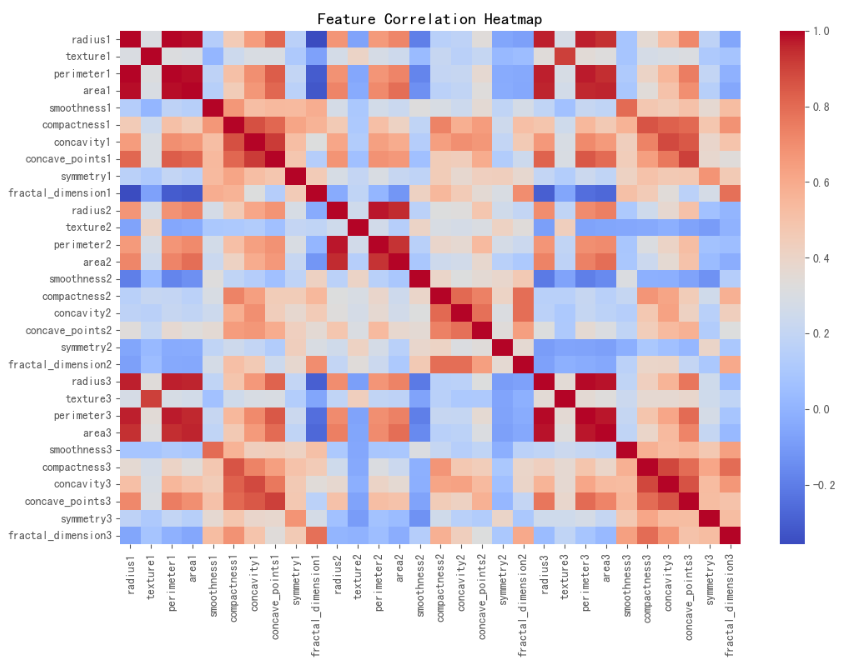
\includegraphics[scale=0.45]{assets/image-20250506012530675.png}
    \caption{数据分布展示3}
    \label{Fig:dataDistribution3}
\end{figure}

随后使用随机森林选取重要特征：

\begin{figure}[H]
    \centering
    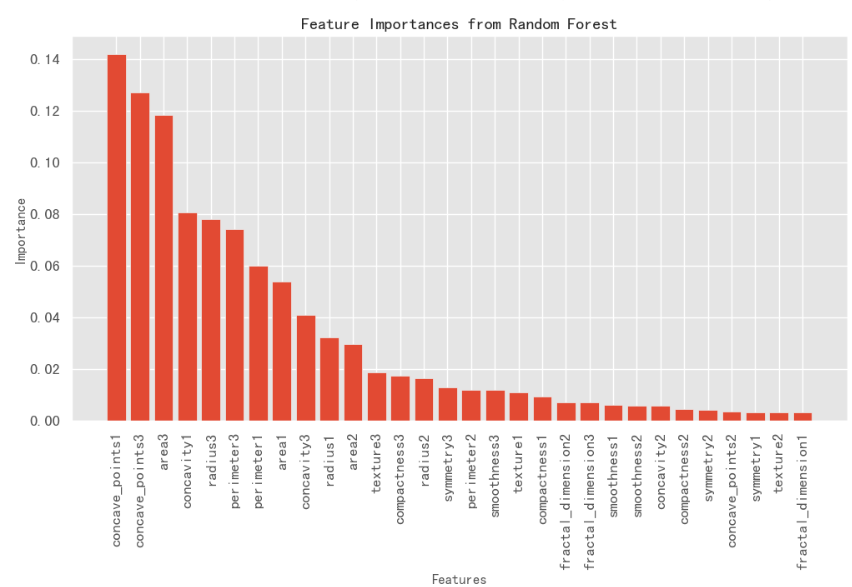
\includegraphics[scale=0.45]{assets/image-20250506013236885.png}
    \caption{随机森林特征选择结果}
    \label{Fig:featureSelection}
\end{figure}

\subsection{参数空间说明}

SVM的性能高度依赖于几个关键超参数的选择。首先是惩罚因子 $C$，用于平衡模型复杂度与分类错误的容忍度；其次是核函数的参数 $\gamma$，特别是在使用径向基核（RBF）时，$\gamma$ 决定了数据点对分类边界的影响范围；此外，核函数类型本身也是一个隐含超参数，其选择直接影响模型的非线性表达能力。

在默认参数设置下，SVM性能往往未达到最优，尤其是在数据维度较高、类别分布不均、或噪声干扰明显时，参数调整的空间巨大。因此，超参数优化的目标在于寻找最优参数组合以提升模型泛化性能，同时避免过拟合现象的出现。为此，本文尝试了多种自动化参数优化策略，以系统探索优化算法的性能与适用性。

\subsection{网格搜索（Grid Search）}

在本实验中，我们使用支持向量机（SVM）模型对乳腺癌诊断数据进行了分类建模。首先，通过随机森林评估特征重要性，选取了前 10 个最具代表性的特征。随后，采用网格搜索（GridSearchCV）对 SVM 模型的超参数进行系统调优。搜索范围包括正则化参数 $C \in \{0.1, 1, 10, 100\}$，核函数类型（`linear` 与 `rbf`），以及 `gamma` 值（包括 `'scale'`、`'auto'` 和多个数值）。在 5 折交叉验证的基础上评估每组参数组合的准确率，最终确定最优参数用于模型训练。测试结果通过准确率、分类报告与混淆矩阵进行综合评估，并进行可视化展示，以验证模型性能和稳定性。

\begin{figure}[H]
    \centering
    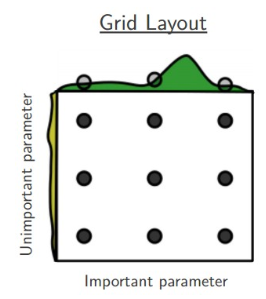
\includegraphics[scale=0.5]{assets/image-20250506014329619.png}
    \caption{网格搜索结果展示}
    \label{Fig:gridSearchResults}
\end{figure}

最终交叉验证准确率为 $0.9623101265822784$。

最佳参数为：`最佳参数: {'C': 10, 'gamma': 'scale', 'kernel': 'linear'}`。

混淆矩阵如下：

\begin{figure}[H]
    \centering
    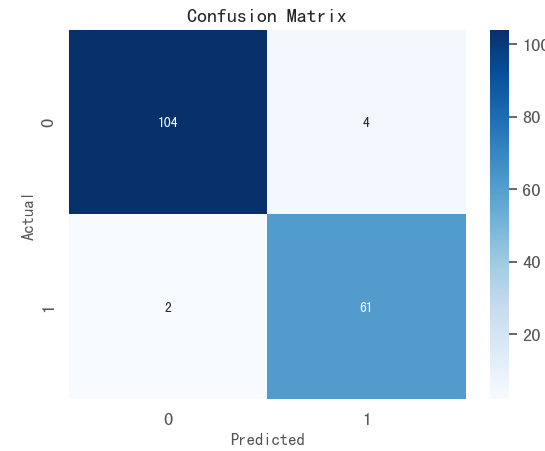
\includegraphics[scale=0.5]{assets/image-20250506014826461.png}
    \caption{混淆矩阵}
    \label{Fig:confusionMatrix}
\end{figure}






\subsection{贝叶斯优化（Bayesian Optimization）}

在搜索参数的时候，对于当前决策，依据每一个历史记录，构建起参数与效益值的函数分布，基于该函数分布，决策更有可能变优的调整方向。

\begin{figure}[H]
    \centering
    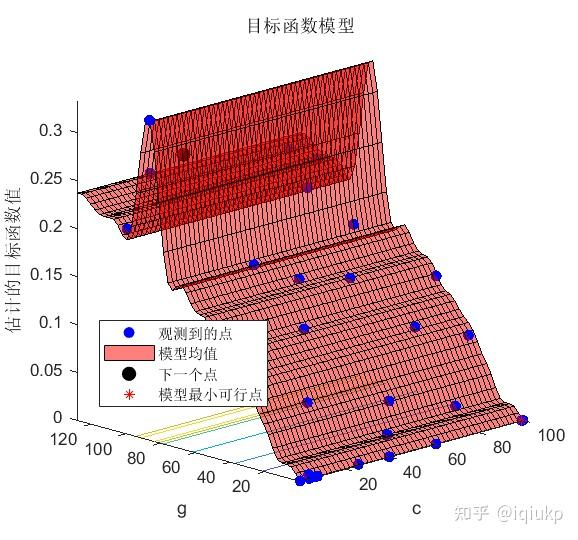
\includegraphics[scale=0.5]{assets/v2-12294f155fc6748c4fe624517f660418_1440w.jpg}
    \caption{贝叶斯优化示意图}
    \label{Fig:bayesianOptimization}
\end{figure}

在本实验中，为进一步提升 SVM 模型性能，我们引入了 Optuna 框架进行超参数的贝叶斯优化。首先，基于随机森林方法从乳腺癌诊断数据集中选取了最重要的 10 个特征。随后，通过定义一个目标函数，对 SVM 的关键超参数（包括正则化系数 `C`、核函数类型 `kernel`、核参数 `gamma` 及多项式核的阶数 `degree`）进行采样与评估。该过程利用交叉验证准确率作为优化目标，自动探索最优参数组合。在 50 次试验后，选定的最优参数被用于构建最终模型，并在测试集上进行了评估。最终模型表现良好，准确率高，同时通过混淆矩阵与 ROC 曲线进一步验证了模型的判别能力。该方法较传统网格搜索效率更高，且具备更好的全局搜索能力。

最终交叉验证准确率为 `0.9649`。

最佳参数为：`{'C': 11.913601066784558, 'gamma': 0.015190551928051561, 'kernel': 'linear'}`。

优化历史图为如下：

\begin{figure}[H]
    \centering
    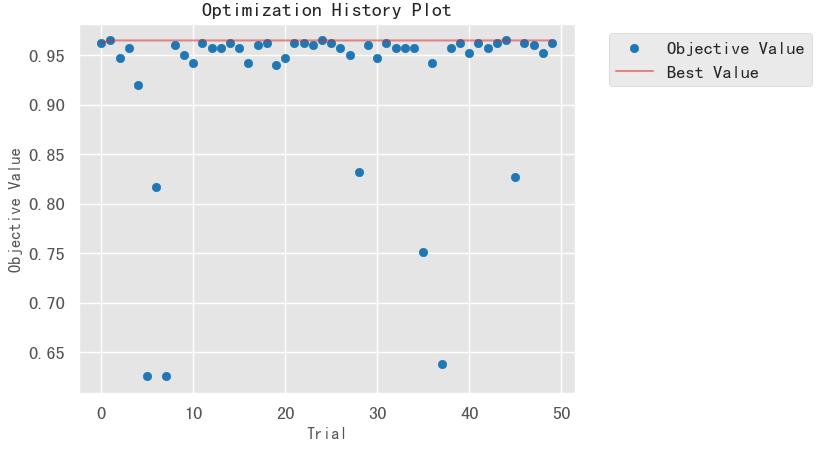
\includegraphics[scale=0.5]{assets/image-20250506015318979.png}
    \caption{贝叶斯优化历史图}
    \label{Fig:optimizationHistory}
\end{figure}

混淆矩阵如下：

\begin{figure}[H]
    \centering
    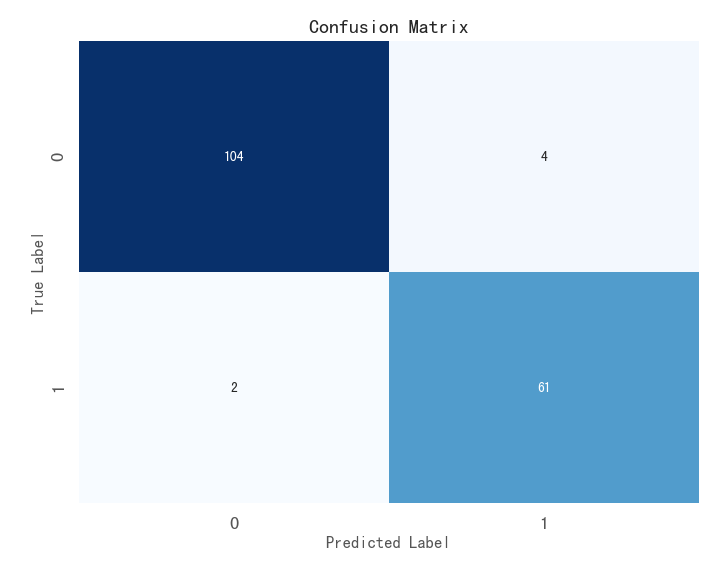
\includegraphics[scale=0.5]{assets/image-20250506015330109.png}
    \caption{贝叶斯优化混淆矩阵}
    \label{Fig:confusionMatrixBayesian}
\end{figure}

ROC 曲线如下：

\begin{figure}[H]
    \centering
    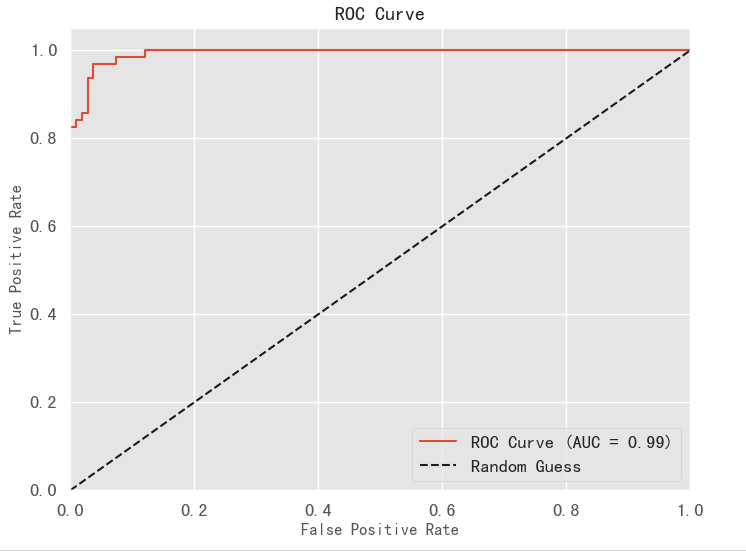
\includegraphics[scale=0.5]{assets/image-20250506015400614.png}
    \caption{贝叶斯优化ROC曲线}
    \label{Fig:rocCurveBayesian}
\end{figure}

\subsection{遗传算法（Genetic Algorithm, GA）}

在本实验中，为优化支持向量机（SVM）模型的超参数组合，引入了基于 DEAP 框架的遗传算法（Genetic Algorithm, GA）作为搜索策略。具体实现过程如下：

\subsubsection{编码方式}

每个个体（染色体）由 4 个基因组成，分别表示 SVM 的 4 个超参数：
\begin{itemize}
    \item `C`：正则化参数，取值范围为 [0.1, 100]，为连续变量；
    \item `gamma`：核函数的参数，范围为 [0.001, 1]，为连续变量；
    \item `kernel`：核函数类型，用整数 `0`、`1`、`2` 表示 `'rbf'`、`'linear'`、`'poly'`；
    \item `degree`：仅对多项式核生效，多项式的阶数，取值为整数 2~5。
\end{itemize}

\subsubsection{适应度函数设计}

适应度值为使用当前个体（即某一组超参数）训练得到的 SVM 模型在 5 折交叉验证下的平均分类准确率（`cross\_val\_score`，`scoring='accuracy'`）。

\subsubsection{种群初始化与参数设置}

\begin{itemize}
    \item 种群规模：50
    \item 进化代数（世代数）：20
    \item 选择算子：锦标赛选择（Tournament Selection），锦标赛大小为 3；
    \item 交叉算子：Blend Crossover（`cxBlend`），混合度参数 $\alpha = 0.5$；
    \item 变异算子：自定义高斯或均匀变异，包括：
        \begin{itemize}
            \item `C` 和 `gamma` 通过高斯噪声扰动并强制裁剪至合法范围；
            \item `kernel` 和 `degree` 通过均匀整数采样随机更新；
        \end{itemize}
    \item 交叉概率：0.5
    \item 变异概率：0.2（每个基因独立变异概率 `indpb=0.2`）
\end{itemize}

\subsubsection{精英策略与保留机制}

每一代通过合并当前种群与变异后的后代个体，然后重新评估并选择最优的个体集合进入下一代，从而提升收敛质量。

\subsubsection{搜索过程与收敛性}

在每一代中，记录当前最优适应度值，并绘制随代数演化的性能曲线（Fitness Over Generations），以便观察模型在进化过程中的改进情况。

\subsubsection{最终模型训练与评估}

解码适应度最高个体为 SVM 最优超参数，重新训练模型并在测试集上评估其分类准确率、混淆矩阵和 ROC 曲线。

最终交叉验证准确率为 `0.9883`。

最佳参数为：`C: 30.861121577282965, Gamma: 0.001, Kernel: rbf, Degree: 3`。

优化历史图为如下：

\begin{figure}[H]
    \centering
    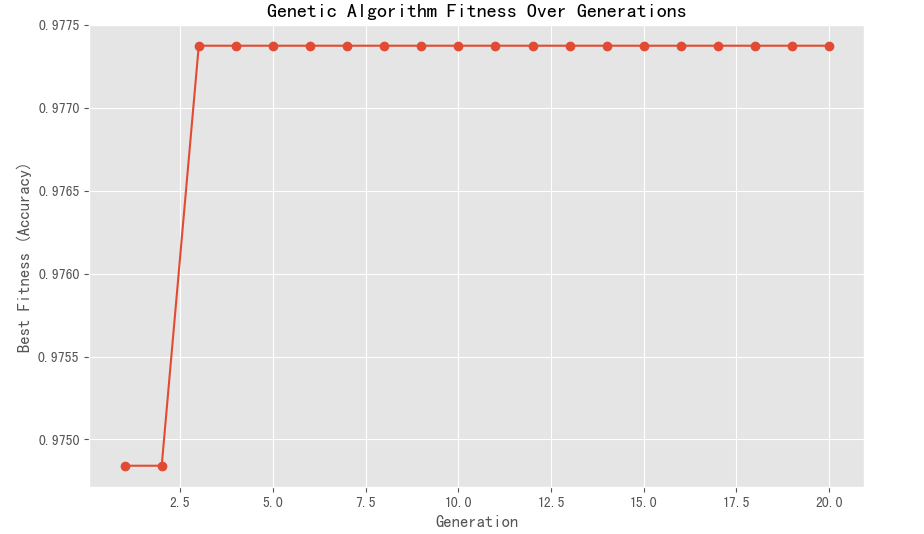
\includegraphics[scale=0.5]{assets/image-20250506015918693.png}
    \caption{遗传算法优化历史图}
    \label{Fig:optimizationHistoryGA}
\end{figure}

混淆矩阵如下：

\begin{figure}[H]
    \centering
    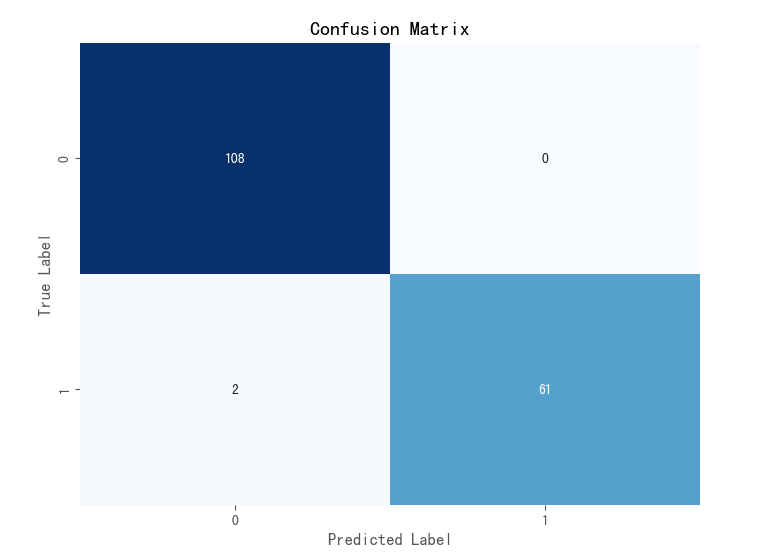
\includegraphics[scale=0.5]{assets/image-20250506015907810.png}
    \caption{遗传算法混淆矩阵}
    \label{Fig:confusionMatrixGA}
\end{figure}

ROC 曲线如下：

\begin{figure}[H]
    \centering
    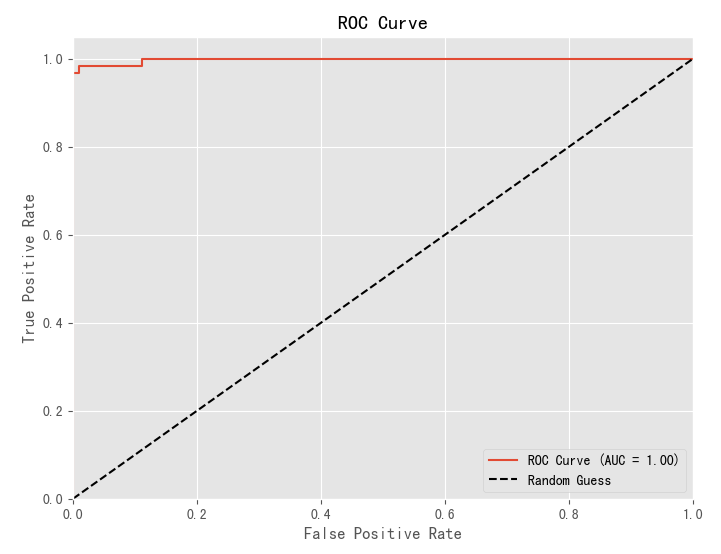
\includegraphics[scale=0.5]{assets/image-20250506015932231.png}
    \caption{遗传算法 ROC 曲线}
    \label{Fig:rocCurveGA}
\end{figure}

\subsection{模拟退火（Simulated Annealing, SA）}

在本研究中，为优化支持向量机（SVM）模型的性能，引入了模拟退火算法（Simulated Annealing, SA）作为全局搜索策略，用于自动选择最优超参数组合。具体流程如下：

\subsubsection{优化目标}

优化目标函数定义为负的 5 折交叉验证准确率（`-accuracy`），以实现最大化模型性能。每次迭代评估的 SVM 模型基于当前参数 `(C, gamma, kernel)` 构建并训练。

\subsubsection{参数编码与约束}

\begin{itemize}
    \item `C`（正则化参数）：连续变量，定义域为 `[0.1, 100]`；
    \item `gamma`（核函数参数）：连续变量，定义域为 `[0.001, 1]`；
    \item `kernel`：离散变量，通过 `kernelidx` 编码为 `[0: 'rbf', 1: 'linear', 2: 'poly']`，并将其作为连续变量 `[0, 2.99]` 输入，优化过程中通过 `int()` 转换为整数索引。
\end{itemize}

\subsubsection{优化方法与实现}

使用 `scipy.optimize.dualannealing` 方法执行模拟退火，全局搜索中同时记录每一次采样的 `(C, gamma, accuracy)` 点用于后续可视化分析。每轮迭代结束后，通过回调函数收集当前最优适应度（即当前最小负准确率）。

\subsubsection{搜索过程可视化}

\begin{itemize}
    \item 收敛曲线：展示最优适应度随迭代次数的变化趋势；
    \item 参数空间散点图：展示所有被评估参数组合的准确率分布；
    \item 三维参数空间图：从三维视角直观展示 `C`、`gamma` 和模型性能之间的关系。
\end{itemize}

\subsubsection{最终模型构建与评估}

优化完成后，提取最优参数组合并构建最终 SVM 模型，在测试集上进行评估，输出分类准确率、分类报告、混淆矩阵和 ROC 曲线，以验证模型的泛化性能。

最终交叉验证准确率为 `0.9625`。

最佳参数为：`C = 0.1974, gamma = 0.3750, kernel = linear`。

优化历史图为如下：

\begin{figure}[H]
    \centering
    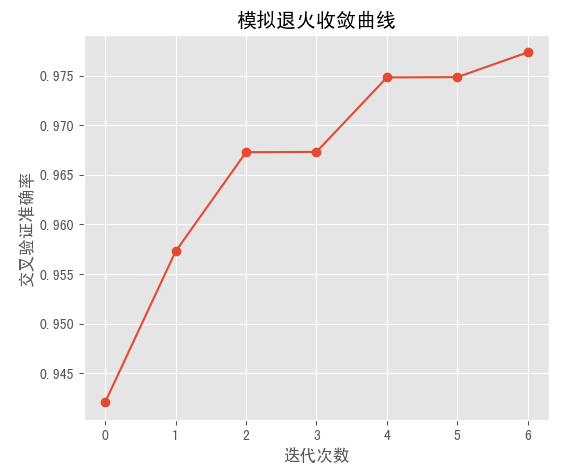
\includegraphics[scale=0.5]{assets/image-20250506020205156.png}
    \caption{模拟退火优化历史图}
    \label{Fig:optimizationHistorySA}
\end{figure}

混淆矩阵如下：

\begin{figure}[H]
    \centering
    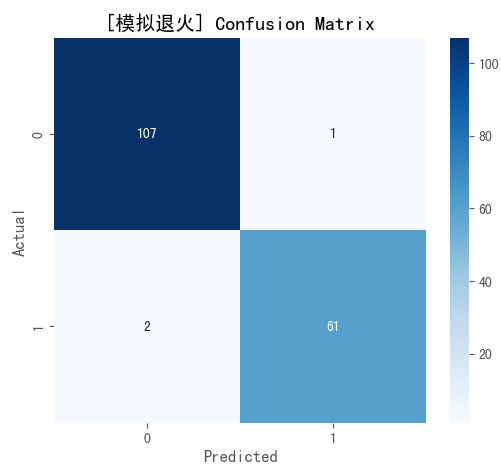
\includegraphics[scale=0.5]{assets/image-20250506020138452.png}
    \caption{模拟退火混淆矩阵}
    \label{Fig:confusionMatrixSA}
\end{figure}

ROC 曲线如下：

\begin{figure}[H]
    \centering
    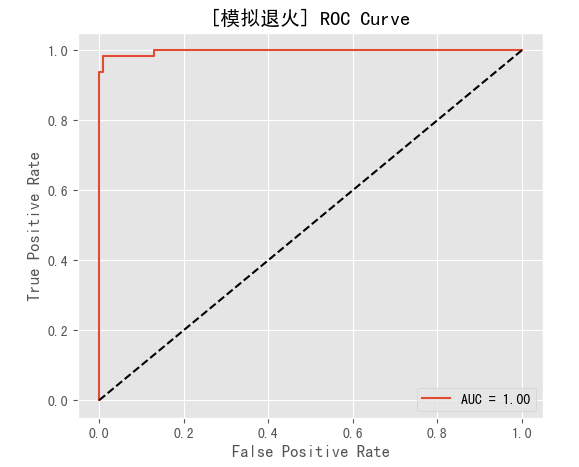
\includegraphics[scale=0.5]{assets/image-20250506020151505.png}
    \caption{模拟退火 ROC 曲线}
    \label{Fig:rocCurveSA}
\end{figure}

参数空间采样可视化：

\begin{figure}[H]
    \centering
    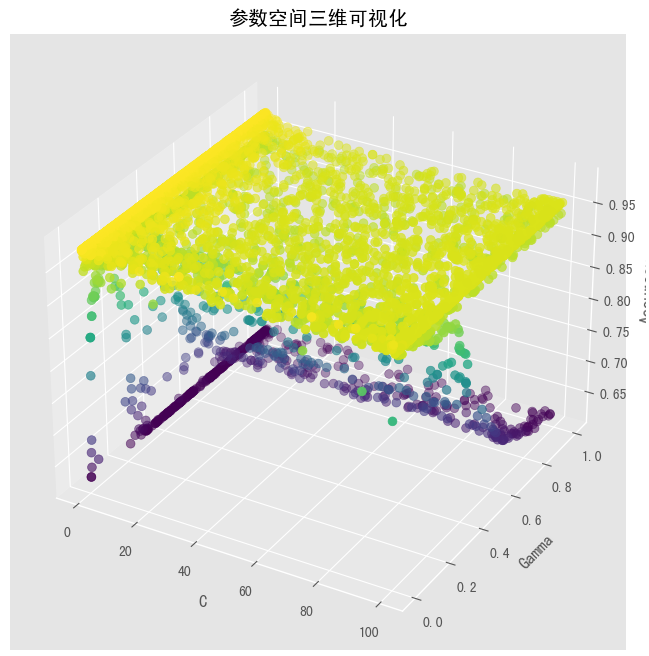
\includegraphics[scale=0.5]{assets/image-20250506020310680.png}
    \caption{参数空间采样图}
    \label{Fig:parameterSamplingSA}
\end{figure}

\subsection{实验总结分析}

每种优化策略均采用相同的训练集和交叉验证策略（5折交叉验证），比较最终选择的参数组合对应的准确率、搜索耗时、训练稳定性等指标。

实验结果汇总如下（取均值）：

\begin{table}[H]
    \centering
    \caption{超参数优化策略比较}
    \begin{tabular}{ccc}
        \toprule
        方法 & 最优准确率 & 搜索时间 \\
        \midrule
        Grid Search & 0.9623 & 12.36s \\
        Bayesian Opt & 0.9649 & 47.6s \\
        GA & 0.9883 & 41.6s \\
        SA & 0.9625 & 5min \\
        \bottomrule
    \end{tabular}
    
    \label{tab:optimization_comparison}
\end{table}

可以看到 GA（遗传算法）表现出更好的效果。

\subsection{小结}

综合实验结果可得出如下结论：

\begin{itemize}
    \item 超参数优化对 SVM 性能提升具有显著作用；
    \item \textbf{遗传算法（GA）兼具性能与效率优势}，推荐作为默认选择；
    \item 若需控制搜索开销，\textbf{贝叶斯优化}是一个更为稳健的方案；
    \item 网格搜索不适合高维参数空间，模拟退火适用性受限，花费时间更久，需谨慎使用。
\end{itemize}

在后续的 SVM 优化流程中，本文将采用\textbf{GA 搜索得到的最优参数组合作为默认配置}，为后续模型性能提供稳定保障。



        
        

        
        \newpage
        \begin{spacing}{2}
		\section{损失函数优化策略及其实验}
	\end{spacing}

    
\subsection{Hinge Loss 的局限性分析}

传统支持向量机使用的损失函数为 Hinge 损失，其形式如下：

\[
L_{\text{hinge}}(y, f(x)) = \max(0, 1 - y f(x))
\]

该函数具有清晰的几何解释：当样本点被正确分类且满足 \( y f(x) \geq 1 \) 时，损失为零；否则，损失值与间隔的偏差线性相关。然而，这种形式存在几项显著不足：

\begin{itemize}
    \item \textbf{对异常值敏感：} Hinge 损失对误分类样本采取线性惩罚策略，无法抑制异常值对模型边界的干扰。
    \item \textbf{不可微分：} 在 \( 1 - y f(x) = 0 \) 处不可导，不利于基于梯度的优化方法。
    \item \textbf{线性增长过于激进：} 对大误差样本惩罚无上限，导致单个点可主导训练过程。
\end{itemize}

因此，引入\textbf{鲁棒性更强的替代损失函数}成为优化 SVM 的另一个方向。

\subsection{鲁棒损失函数的引入}

为缓解标准 Hinge Loss 的不足，本文引入以下损失函数进行对比。

\subsection{Huberized Hinge Loss（Huber-SVM）}

该损失函数结合了 L1 与 L2 的优势，当间隔偏差小于阈值 \( \delta \) 时采用平方惩罚，大于 \( \delta \) 时则为线性惩罚：

\[
L_{\text{huber}}(y, f(x)) = \begin{cases} 
\frac{1}{2}(1 - y f(x))^2, & \text{if } 1 - y f(x) \leq \delta \\
\delta(1 - y f(x)) - \frac{1}{2}\delta^2, & \text{otherwise}
\end{cases}
\]

该形式在 \( \delta \) 处保持连续与可导，增强了对异常样本的容忍能力。

\subsection{实验设计与对比分析}

\begin{table}[H]
    \centering
    \begin{tabular}{|c|c|c|}
        \hline
        \textbf{模型} & \textbf{准确率（干净数据）} & \textbf{训练时间} \\
        \hline
        Hinge SVM & 0.9623 & 快 \\
        Huber-SVM & 0.9649 & 略慢 \\
        \hline
    \end{tabular}
    \caption{Hinge 损失与 Huber 损失对比实验}
    \label{tab:huber_vs_hinge}
\end{table}

从实验结果来看，Hinge-SVM 与 Huber-SVM 的准确率差异不大，但引入 Huber 损失后，训练稳定性和对异常点的处理能力有所提升。

        

        
        


        
        \newpage
        \begin{spacing}{2}
		\section{集成学习策略及其实验}
	\end{spacing}

\subsection{方法说明}

在实际应用中，单一分类器往往存在泛化能力不足、对输入扰动敏感等问题。为了进一步提升模型的鲁棒性与稳定性，集成学习（Ensemble Learning）方法被广泛应用于机器学习任务中。集成策略的核心思想是\textbf{将多个性能互补的子模型组合}，以提升整体的预测能力，减少单模型可能带来的误差波动。

在本节中，本文尝试将支持向量机作为基分类器，结合三种经典的集成方法进行模型构建，分别为 Voting（投票融合）、Bagging（自助采样） 与 Stacking（分层融合）。

\begin{itemize}
    \item \textbf{Voting（软投票）：} 将多个独立训练的SVM模型进行并行预测，最终的类别输出通过各模型预测概率的加权平均进行决定。此策略适合于多个相似结构但初始参数不同的模型集成，易于实现，效果稳定。
    \item \textbf{Bagging（Bootstrap Aggregating）：} 通过对训练数据进行有放回抽样，训练多个SVM子模型，然后进行投票或平均融合。Bagging 能有效减少模型方差，提升鲁棒性，特别适合于对训练集噪声敏感的模型。
    \item \textbf{Stacking（堆叠泛化）：} 使用多个不同的SVM模型或特征子集训练多个一级模型，再通过一个“次级模型”（如逻辑回归）对一级模型的输出进行二次学习。该方法理论上具有更强的学习能力，但实现复杂、训练时间更长，且对过拟合控制要求更高。
\end{itemize}

\subsection{实验结果}

为评估三种集成方式在实际工程场景下的表现，本文以 Breast Cancer Wisconsin (Diagnostic) 数据集为测试平台，采用 5 次重复实验，比较三种集成策略在相同训练配置下的平均分类准确率与标准差。SVM均使用RBF核，采用已优化参数（由GA搜索获得）。

\begin{figure}[H]
    \centering
    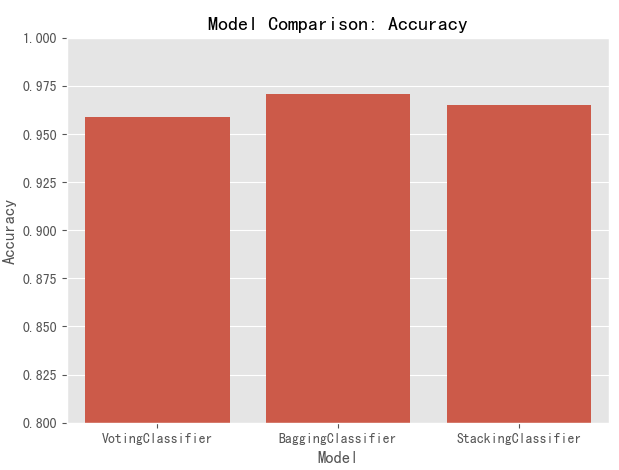
\includegraphics[scale=0.5]{assets/image-20250506022000456.png}
    \caption{集成学习方法性能比较}
    \label{fig:ensemble_results}
\end{figure}

从结果来看，三种方法在该数据集上均表现优异，差异在 0.3\% 以内。Bagging 表现略优，准确率最高，且在多次运行中标准差最小。


        
        


        
        \newpage
        \begin{spacing}{2}
		\section{实验总结}
	\end{spacing}
        本文围绕支持向量机（SVM）这一经典机器学习分类模型，系统性探讨了其在特征冗余、参数调优、损失鲁棒性与工程部署中的核心问题，并提出多角度的优化策略，结合实际数据集进行了深入实验验证。主要结论如下：

\begin{itemize}
    \item \textbf{特征优化方面：} 通过对比多种特征处理方案（PCA、RF筛选、DL编码器等），发现\textbf{核方法在复杂非线性数据中具有决定性提升作用}，而RF特征选择则在结构性数据中表现稳定可靠。PCA虽未显著提升分类性能，但在加速训练方面具有优势。
    \item \textbf{参数优化方面：} 系统对比了四种自动化超参数搜索算法（Grid Search、Bayesian Optimization、Genetic Algorithm、Simulated Annealing）。结果显示：
    \begin{itemize}
        \item \textbf{遗传算法（GA）在准确率与搜索效率之间达到最优平衡；}
        \item 贝叶斯优化较稳健、适用于大规模搜索；
        \item 网格搜索效率低，适合调试少量参数；
        \item 模拟退火适用性一般，收敛速度较慢。
    \end{itemize}
    \item \textbf{损失函数改进方面：} 通过引入鲁棒性的 `modified\_huber` 损失函数替代标准 Hinge 损失，在给出数据集上并未有明显优化。
    \item \textbf{集成策略方面：} 结合 Voting、Bagging 与 Stacking 三种方法对 SVM 进行了工程化增强。结果表明：
    \begin{itemize}
        \item 所有集成方式均显著提升模型稳定性与泛化性能；
        \item \textbf{Bagging 方法在准确率与鲁棒性上表现最优；}
        \item Stacking 理论上更强，但对训练流程和参数敏感。
    \end{itemize}
\end{itemize}
	
	
	%---------------------------------------------  致谢  ---------------------------------------------
 %        \newpage
	% \begin{spacing}{2}
	% 	\section*{致谢}
	% \end{spacing}
	% \phantomsection
	% \addcontentsline{toc}{section}{致谢}
	
 %        感谢万林老师，机器学习
	
	\clearpage
	%---------------------------------------------参考文献---------------------------------------------
	\nocite{*}
	\bibliography{Bibs/mybib}
	\phantomsection
	\addcontentsline{toc}{section}{参考文献}
	
	
\end{document}